%ju 28-Mai-22 FM_U05_Innenwiderstand_Loesung.tex
\section{Innenwiderstand Übung 5}\label{innenwiderstand-uebung-5}

\textbf{Aufgabe 1}

Ein $24~V$ Starter wird über zwei $12~V$ Batterien mit elektrischer
Energie versorgt. Die Batteriezellen besitzen einen Innenwiderstand von
$0,74~m\Omega$/Zelle. Durch die $2,3~m$ lange Versorgungsleitung mit
einer Fläche von $120~mm^2$ fließt ein Strom von $1250~A$.

Wie groß ist die Klemmenspannung am Starter?

\begin{figure}[!ht]% hier: !ht
\centering
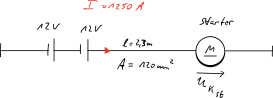
\includegraphics[width=0.6\textwidth]{images/Skizze/20_FM_Nr5_Innenwiderstand_Aufg1_Skizze.pdf}
\caption{Schaltung Innenwiderstand Aufgabe 1}
%\label{fig:}%% anpassen
\end{figure}

geg:

$R_{i_{zelle}} = 0,00074~\Omega = 0,74~m \Omega /Zelle$

$U_{{Bat}_1} = 12~V$

$U_{{Bat}_2}= 12~V$

$z = 12$ (Anzahl Batteriezellen)

$I = 1250~A$

$l = 2,3~m$

$A = 120~mm^2$

$\rho = 0,0178~\frac{\Omega \cdot mm^2}{m}$

ges: $U_{K_{st}}$

Formel:

$U_i = R_{i_{ges}} \cdot I \quad \to U_i = R_{i_{zelle}} \cdot z \cdot I$

$U_v = \frac{I \cdot \rho \cdot l}{A}$

$U_{ges} = U_i + U_v + U_{K_{st}} \quad \to U_{K_{st}} = U_{{Bat}_1} + U_{{Bat}_2} - U_v - U_i$

Lösung:

$U_i = 11,1~V$

$U_v = 0,4265~V$

$U_{K_{st}} = 12,4735~V$

\textbf{Aufgabe 2}

\begin{figure}[!ht]% hier: !ht
\centering
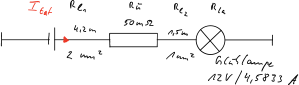
\includegraphics[width=0.6\textwidth]{images/Skizze/21_FM_Nr5_Innenwiderstand_Aufg2_Skizze.pdf}
\caption{Schaltung Innenwiderstand Aufgabe 2}
%\label{fig:}%% anpassen
\end{figure}

geg: Glühlampenaufschrift: $12~V / 4,5833~A$

$U = 12~V$

$I = 4,5833~A$

$U_q = 14,8~V$

$R_i = 0,012~\Omega = 12~m \Omega$

$A_1 = 2~mm^2, A_2 = 1~mm^2$

$l_1 = 4,2~m, l_2 = 1,5~m$

$R_\text{ü} = 0,050~\Omega = 50~m \Omega$

$\rho = 0,0178~\frac{\Omega \cdot mm^2}{m}$

ges: Mit welcher Klemmenspannung wird die Schaltung gespeist?

Formel:

$R_{l_1} = \frac{\rho \cdot l_1}{A_1}, R_{l_2} = \frac{\rho \cdot l_2}{A_2}$

$R_{La} = \frac{U}{I}$

$R_{ges} = R_i + R_{l_1} + R_\text{ü} + R_{l_2} + R_{La}$

$I_{tat} = \frac{U_q}{R_{ges}}$

$U_K = U_q - I \cdot R_i$

Lösung:

$R_{l_1} = 0,0374~\Omega, R_{l_2} = 0,0267~\Omega$

$R_{La} = 2,6182~\Omega$

$R_{ges} = 2,7443~\Omega$

$I_{tat} = 5,393~A$

$U_K = 14,745~V$
